\documentclass{article}

\usepackage[paperwidth=118.9cm,paperheight=84.1cm,margin=0mm]{geometry}

\usepackage{fontspec}
\usepackage{polyglossia}
\usepackage{tikz}
\usepackage{xcolor}
\usepackage{graphicx}
\setdefaultlanguage{russian}
\setotherlanguage{english}

\setmainfont{DejaVu Sans}
\setsansfont{DejaVu Sans}
\setmonofont{DejaVu Sans Mono}
\newfontfamily\cyrillicfont{DejaVu Sans}
\newfontfamily\cyrillicfontsf{DejaVu Sans}

\pagestyle{empty}
\setlength{\parindent}{0pt}

% ---------- colors ----------
\definecolor{ink}{HTML}{182840}
\definecolor{headerred}{HTML}{D72645}
\definecolor{blue}{HTML}{1E6D93}
\definecolor{teal}{HTML}{2B938A}
\definecolor{orange}{HTML}{FF8A1B}
\definecolor{green}{HTML}{55A842}
\definecolor{purple}{HTML}{B06A9A}
\definecolor{red}{HTML}{EF4B4D}
\definecolor{gray}{HTML}{627086}

\definecolor{fillpink}{HTML}{FDEEF1}
\definecolor{fillblue}{HTML}{EAF2FA}
\definecolor{fillgray}{HTML}{F2F4F9}
\definecolor{fillteal}{HTML}{E8F5F1}
\definecolor{fillorange}{HTML}{FFF2E5}
\definecolor{fillgreen}{HTML}{EEF8EC}
\definecolor{fillpurple}{HTML}{F2EEF9}

% x,y,w,h are in cm; (0,0) = top-left of page.
\newcommand{\posterbox}[7]{%
  \draw[line width=1.4mm, draw=#5, fill=#6]
    ([xshift=#1cm,yshift=-#2cm]current page.north west)
    rectangle ++(#3cm,-#4cm);
  \node[anchor=north west, text=ink, inner sep=0pt,
        font=\bfseries\fontsize{34}{40}\selectfont,
        text width=\dimexpr#3cm-1.6cm\relax]
    at ([xshift=#1cm+0.8cm,yshift=-#2cm-0.8cm]current page.north west) {#7};
}

\newcommand{\smallplot}{%
\begin{tikzpicture}[x=0.48cm,y=0.48cm]
  \draw[gray!55,line width=.35mm] (0,0) rectangle (15,7);
  \draw[gray!35,line width=.2mm] (1.5,1) -- (1.5,6.2);
  \draw[gray!35,line width=.2mm] (1.5,1) -- (14,1);
  \draw[blue,line width=.55mm] (2,1.4)--(5,2.4)--(8,3.5)--(11,4.7)--(13.4,5.7);
  \draw[green,line width=.55mm] (2,1.2)--(5,2.0)--(8,3.0)--(11,4.0)--(13.4,5.0);
  \draw[orange,line width=.55mm] (2,1.6)--(5,2.5)--(8,3.8)--(11,5.0)--(13.4,6.0);
  \foreach \x/\y in {2/1.6,5/2.5,8/3.8,11/5.0,13.4/6.0}{\fill[orange] (\x,\y) circle (1.2mm);}
\end{tikzpicture}%
}

\begin{document}
\begin{tikzpicture}[remember picture,overlay]

% page border
\draw[line width=0.8mm, draw=ink!80]
  ([xshift=0.6cm,yshift=-0.6cm]current page.north west)
  rectangle
  ([xshift=-0.6cm,yshift=0.6cm]current page.south east);

% ---------- HEADER ----------
\posterbox{2.0}{1.6}{115.0}{7.6}{headerred}{fillpink}{}
\fill[headerred] ([xshift=2.0cm,yshift=-1.6cm]current page.north west) rectangle ++(0.8cm,-7.6cm);

\node[
    anchor=north west,
    text=ink,
    inner sep=0pt,
    font=\bfseries\fontsize{52}{60}\selectfont
] at ([xshift=4.0cm,yshift=-2.1cm]current page.north west)
  {Влияние качества Semantic ID на финальные метрики};

\node[
    anchor=north west,
    text=ink,
    inner sep=0pt,
    font=\fontsize{26}{32}\selectfont
] at ([xshift=4.0cm,yshift=-5.3cm]current page.north west)
  {Константин Рядинский \enspace\textbullet\enspace
   Лев Клюев \enspace\textbullet\enspace
   Ростислав Головков \enspace\textbullet\enspace
   Глеб Шевченко};

\node[
    anchor=north west,
    text=gray,
    inner sep=0pt,
    font=\fontsize{22}{27}\selectfont
] at ([xshift=4.0cm,yshift=-7.3cm]current page.north west)
  {Ментор: Александр Новак};

% ---------- LEFT COLUMN ----------
% ---------- LEFT COLUMN ----------

\posterbox
  {2.0}{10.4}
  {37.3}{17.4}
  {blue}{fillblue}
  {Введение}

\node[
    anchor=north west,
    text width=35.5cm,
    align=left
] at ([xshift=2.8cm,yshift=-12.8cm]current page.north west)
{
    {\fontsize{30}{37}\selectfont

    Semantic IDs (SIDs) используются для дискретного представления
    объектов в генеративных рекомендательных системах.

    \vspace{0.5cm}

    При этом качество SID часто оценивается через
    \textbf{\textcolor{blue}{свойства самого представления}},
    которые не обязательно коррелируют с качеством итоговых рекомендаций.

    \vspace{0.5cm}

    \textbf{Цель нашей работы} --- исследовать эту связь:
    сравнить различные методы построения Semantic IDs и определить,
    какие свойства SID действительно отражаются на финальных метриках
    рекомендательной системы.
    }
};
% Вместо \posterbox используем Ti*k*Z-узел с рамкой и заливкой
\posterbox{2.0}{28.8}{37.3}{35.7}{gray}{fillgray}{Бэйзлайны}

\node[
    anchor=north west,
    text=ink,
    inner sep=0pt,
    text width=35.5cm,
    align=left
] at ([xshift=2.8cm,yshift=-31.0cm]current page.north west)
{
{\fontsize{24}{30}\selectfont

\textbf{\textcolor{red}{Генерация без Semantic IDs}}

\vspace{0.25cm}

\textbf{SASRec} --- одна из первых моделей трансформеров, использующая историю
взаимодействий пользователя с айтемами.

\vspace{0.5cm}

\textbf{\textcolor{orange}{Генерация с Semantic IDs}}

\vspace{0.25cm}

\textbf{TIGER-like} --- генеративная рекомендательная модель,
которая авторегрессионно предсказывает последовательность токенов
Semantic ID целевого объекта.

\vspace{0.7cm}

\textbf{\textcolor{blue}{Ранжирование без Semantic IDs}}

\vspace{0.25cm}

В качестве базовых моделей используем стандартные ранжирующие
модели, работающие с обычными \textbf{item ID}:

\vspace{0.35cm}

\textbf{DCNv2} --- надо написать, в чём прикол именно этой модели.

\vspace{0.35cm}

\textbf{TransAct-like} --- надо написать, в чём прикол именно этой модели.

\vspace{0.7cm}

\textbf{\textcolor{teal}{Ранжирование с Semantic IDs}}

\vspace{0.25cm}

Для тех же ранжирующих моделей мы добавляем к обычному индексу объекта
его \textbf{Semantic ID}. Это позволяет напрямую оценить,
как способ построения SID влияет на качество ранжирования.

\vspace{0.7cm}

Таким образом, влияние SID оцениваются как в
\textbf{ранжировании}, так и в \textbf{генерации}.

}
};
\posterbox{2.0}{65.5}{37.3}{16.4}{teal}{fillteal}{Гибкая зона: 1--2 метода после примерки текста (объясните, что это))}

% ---------- RIGHT: methods grid ----------
\posterbox{79.1}{10.4}{37.8}{20.2}{blue}{fillblue}{Balanced RQ-KMeans / RQ-VAE}

\node[anchor=north, inner sep=0pt]
  at ([xshift=98.0cm,yshift=-13.0cm]current page.north west)
  {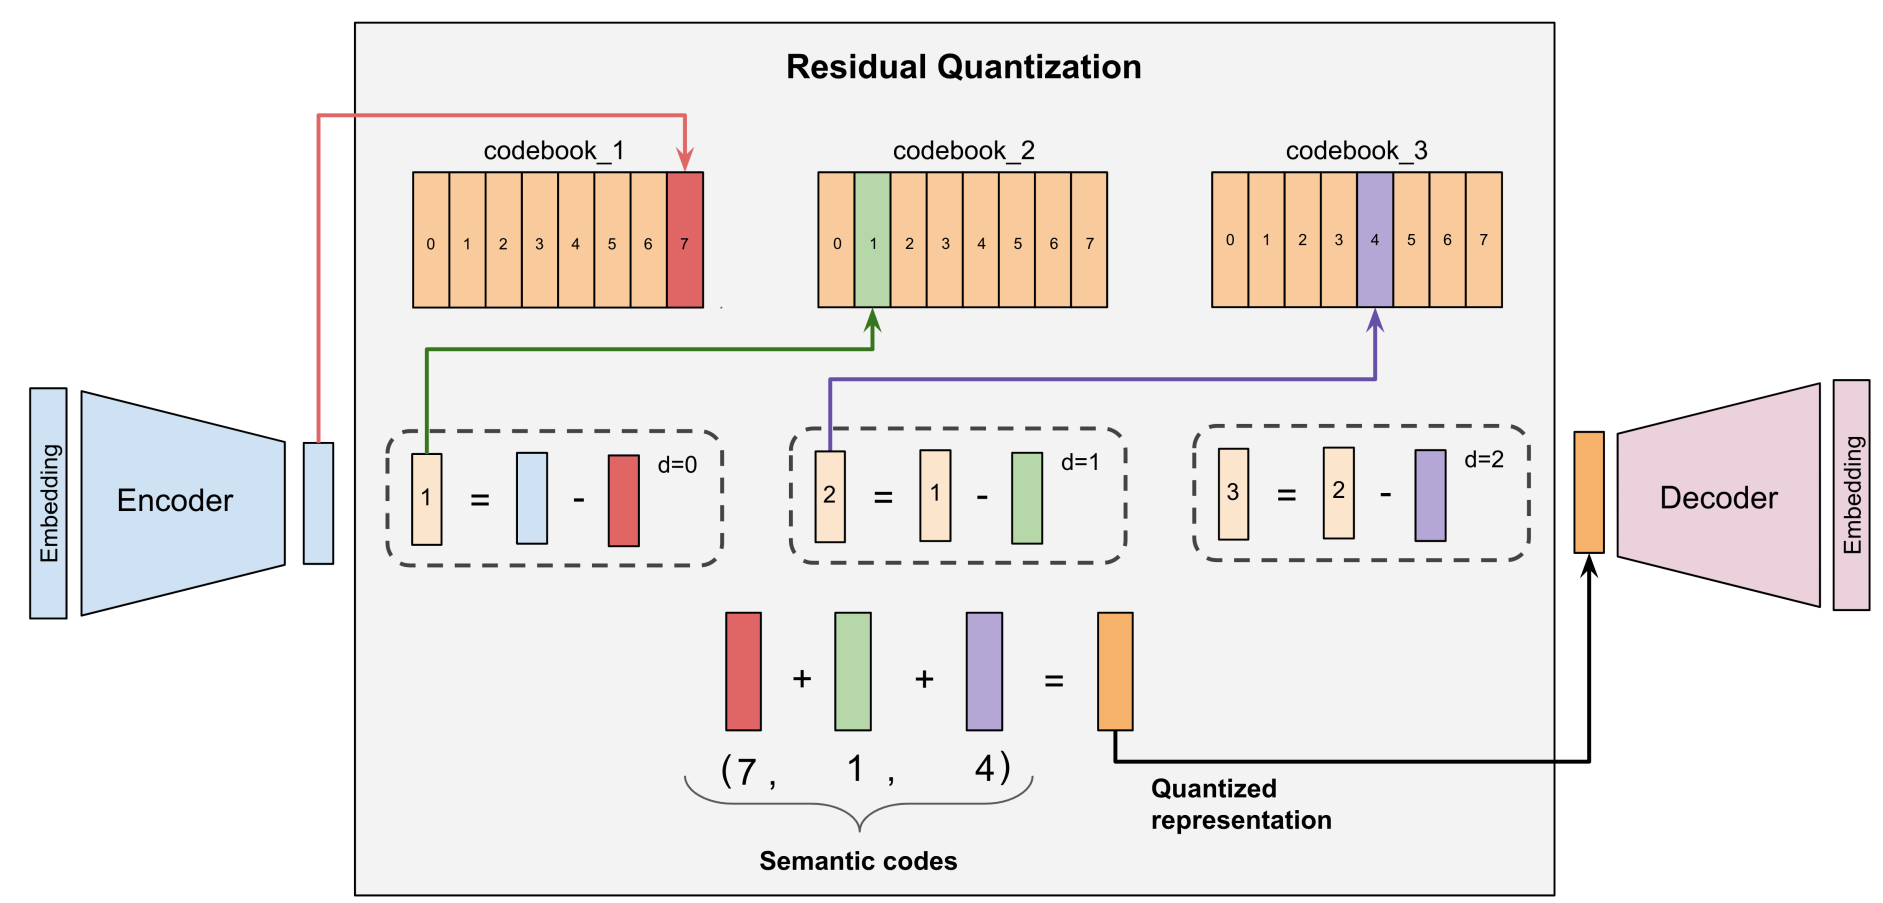
\includegraphics[width=33.5cm]{rq-rqvae.png}};

\node[
    anchor=south east,
    text=gray,
    inner sep=0pt,
    font=\fontsize{11}{13}\selectfont
] at ([xshift=116.1cm,yshift=-30.0cm]current page.north west)
  {Источник: Mike X Cohen (2026), схема Sumit};

\posterbox{79.1}{31.6}{18.4}{16.0}{teal}{fillteal}{PLUM-like}

\node[
    anchor=north west,
    text=ink,
    inner sep=0pt,
    text width=16.8cm,
    align=left
] at ([xshift=79.9cm,yshift=-33.7cm]current page.north west)
{
    {\fontsize{21}{26}\selectfont

    Размер кодбука уменьшается вдвое с каждым уровнем:

    \[
        C_i = \frac{C_0}{2^i}.
    \]

    Случайная \textbf{prefix-маска} выбирает глубину SID:
    обновляются только уровни активного префикса.

    \vspace{0.25cm}

    Последний кодбук используется с вероятностью \textbf{0.25};
    остальные глубины делят оставшуюся вероятность.

    \vspace{0.25cm}

    Ранние уровни обучаются чаще и формируют информативные
    короткие префиксы SID.

    }

};

\posterbox{98.5}{31.6}{18.4}{16.0}{teal}{fillteal}{R3-VAE}

\node[
    anchor=north west,
    text=ink,
    inner sep=0pt,
    text width=16.8cm,
    align=left
] at ([xshift=99.3cm,yshift=-34.0cm]current page.north west)
{
{\fontsize{22}{28}\selectfont
Обучаемый \textbf{reference-вектор} задаёт семантический якорь для начального residual.\\[0.35cm]
\textbf{Dot-product rating} сохраняет поток градиента и предотвращает collapse кодбука.\\[0.35cm]
Регуляризация \textbf{SC/PD} усиливает сходство внутри SID и различия между кластерами.
}
};

\posterbox{79.1}{48.6}{18.4}{15.6}{purple}{fillpurple}{User-aware}
\posterbox{98.5}{48.6}{18.4}{15.6}{orange}{fillteal}{BPE}

\posterbox{79.1}{65.2}{18.4}{16.7}{red}{fillpurple}{PSI}

\node[
    anchor=north west,
    text=ink,
    inner sep=0pt,
    text width=16.8cm,
    align=left
] at ([xshift=79.9cm,yshift=-67.6cm]current page.north west)
{
{\fontsize{22}{28}\selectfont
\textbf{Multi-resolution кодбуки} уменьшаются на глубоких уровнях и компактно кодируют residual.\\[0.35cm]
\textbf{Progressive masking} обучает случайные SID-префиксы, усиливая семантическую иерархию.
}
};

\posterbox{98.5}{65.2}{18.4}{16.7}{purple}{fillteal}{Spectral embeddings}

% ---------- MIDDLE: RESULTS ----------
\posterbox{40.3}{10.4}{37.8}{50.2}{orange}{fillorange}{Эксперименты и графики}
\posterbox{40.3}{61.6}{37.8}{20.3}{headerred}{fillpink}{Главный результат}


\end{tikzpicture}
\null
\end{document}
